\documentclass[a4paper]{article}

%% Language and font encodings
\usepackage[english]{babel}
\usepackage[utf8x]{inputenc}
\usepackage[T1]{fontenc}

%% Sets page size and margins
\usepackage[a4paper,top=3cm,bottom=2cm,left=3cm,right=3cm,marginparwidth=1.75cm]{geometry}

%% Useful packages
\usepackage{amsmath}
\usepackage{graphicx}
\usepackage[colorinlistoftodos]{todonotes}
\usepackage[colorlinks=true, allcolors=blue]{hyperref}

\title{Chapman-Jouguet conditions in ethane-air mixture}
\author{Artur Kuriata}

\begin{document}
\maketitle


\section{Introduction}

Estimating activation energy of explosive mixtures is one of the most difficult cases modern computer fluid dynamics and thermodynamics applied methods.The insufficient computational power limits complexity of differential equations , both in quality and quantity,therefore there is a demand in simplifying  the math while staying accurate with an output.



This report presents study of the CJ conditions in various starting temperatures and pressures.

\section{Model}
Numerical model uses  adiabaticTemp,$cv_CJInd$,explosionInd and finally,activationEnergy
functions to calculate minimal energy needed to activate detonation.Overlooking the reaching to the final formula , the equation for the activation energy is calculated from :

\(E_{a}\approx RT_{0}()(-\frac{T_{0}}{\tau _{i}}\frac{(\tau'_{i}-\tau_{i})}{T'}) +(n+1))\)





Where :

R	->universal gas constant [J/mol/K]

T0 -> 0,9 of starting adiabatic temperature[K]

i -> Chapman – Jouguet induction time in constant volume for T0 [s]

T’ -> slightly larger temperature (T0 + 30) [K]


i’ -> Chapman – Jouguet induction time in constant volume for T’ [s]


n -> effective reaction order, for ethane it equals 3


After calculating approximate activation energy for a few points in explosibility range



Although the output is approximately correct for only narrow range of explosibility around stoichiometric values, it can help in developing explosion preventing systems.


\section{Results}

\hspace{5,5mm} a)Activation energy  at 300 K and 1 atmosphere pressure
\begin{figure}[ht]
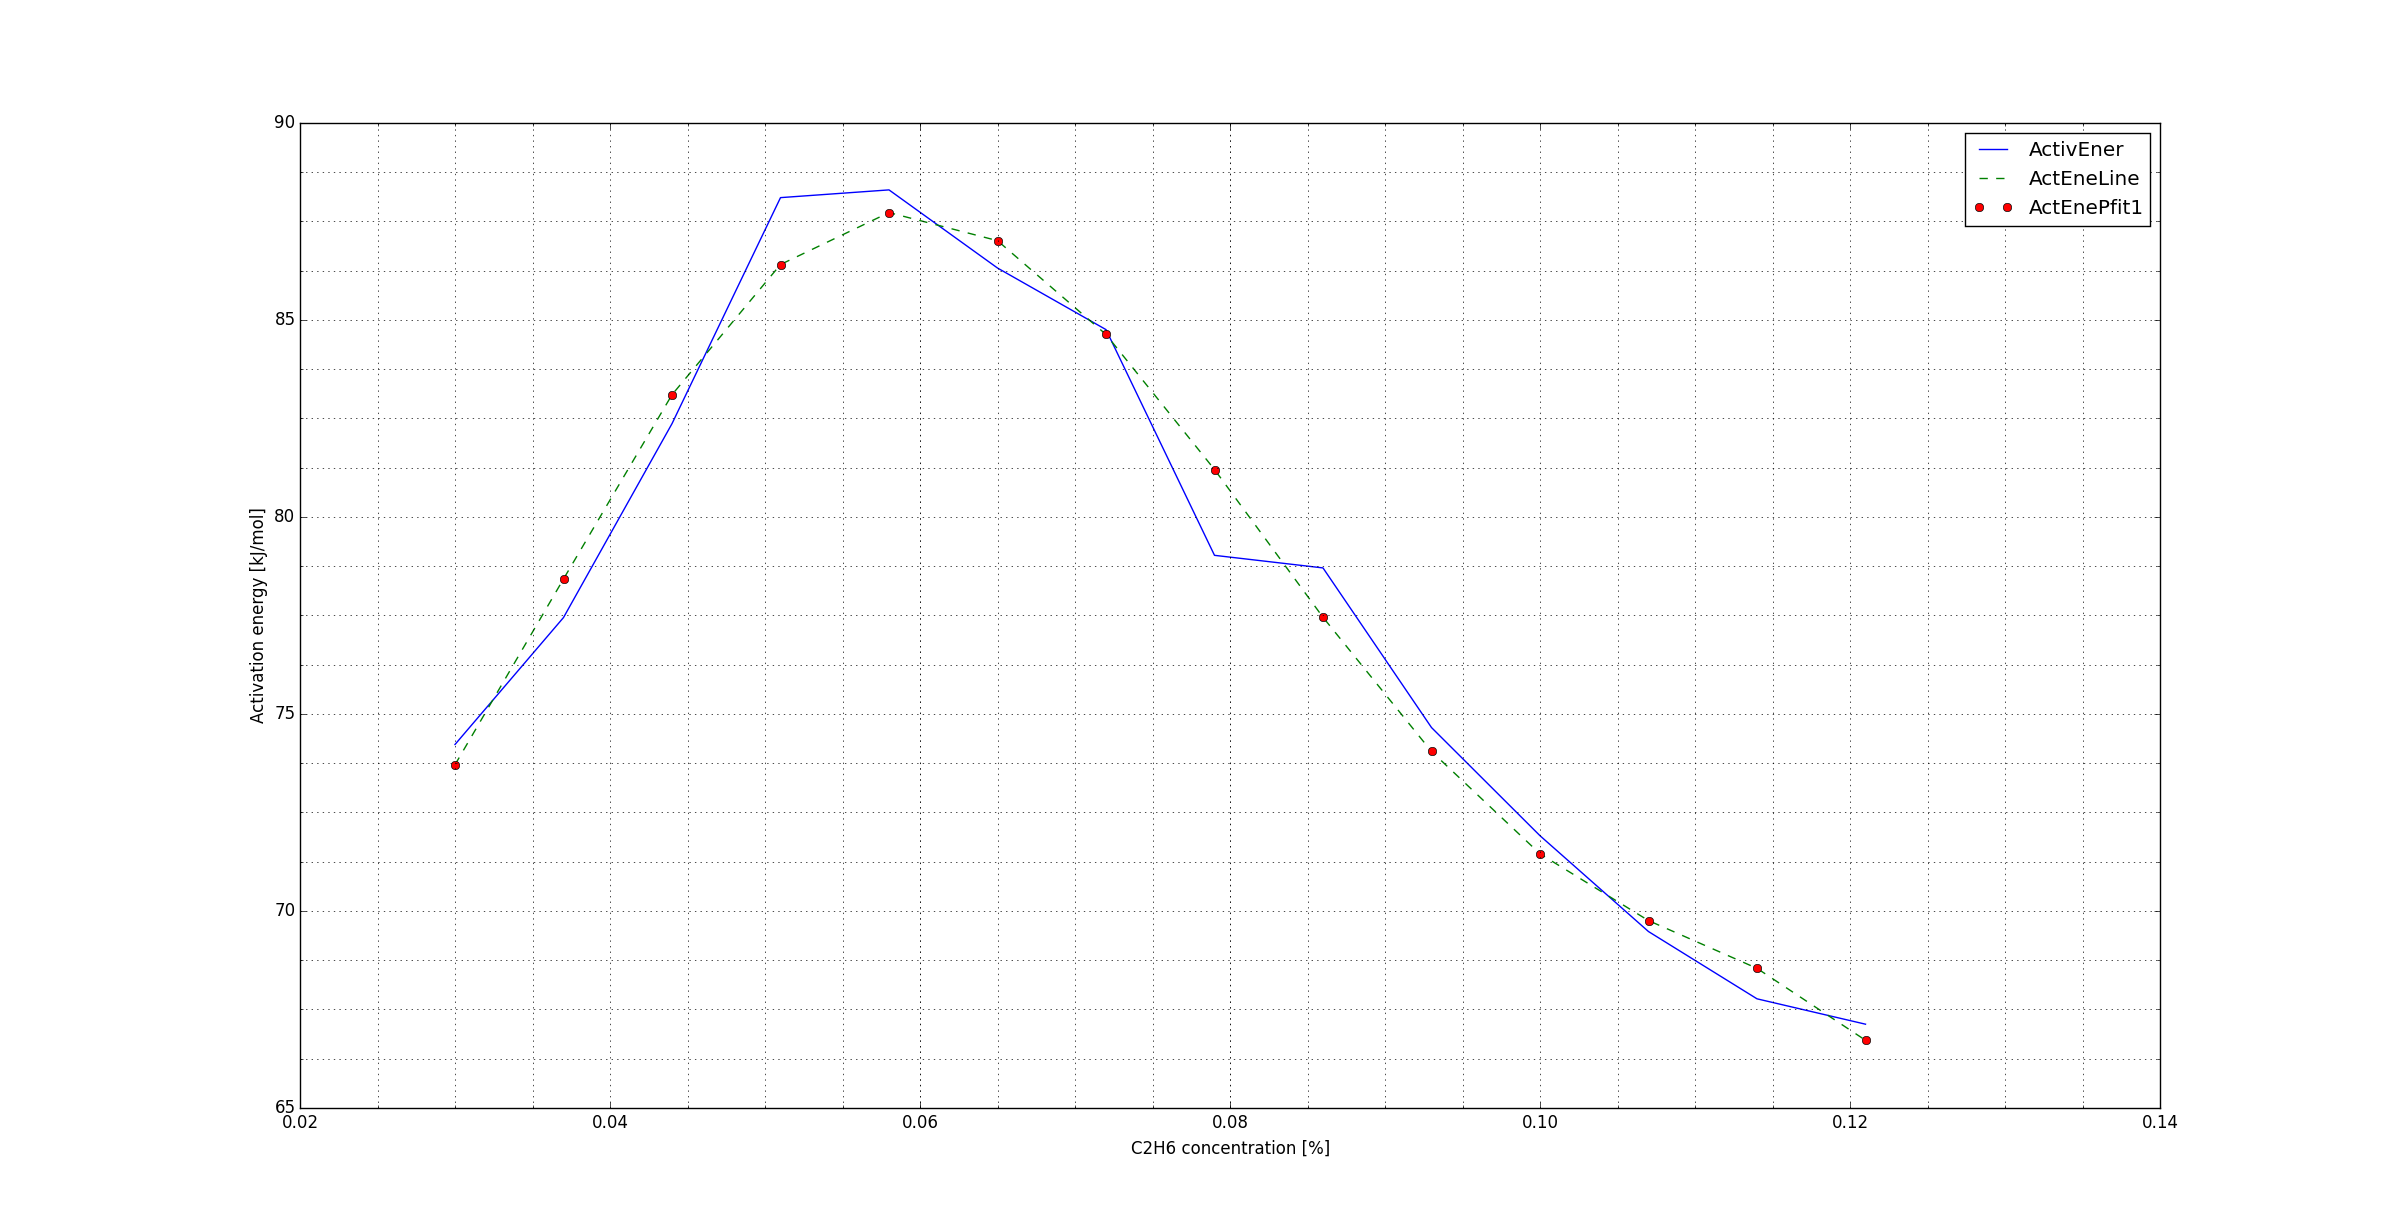
\includegraphics[width=1\textwidth]{figure_1.png}
\caption{Activation energy  at 300 K and 1 atmosphere pressure}
\end{figure}

\hspace{5,5mm} b)Activation energy  at 300 K and 2 atmosphere pressure
\begin{figure}[ht]
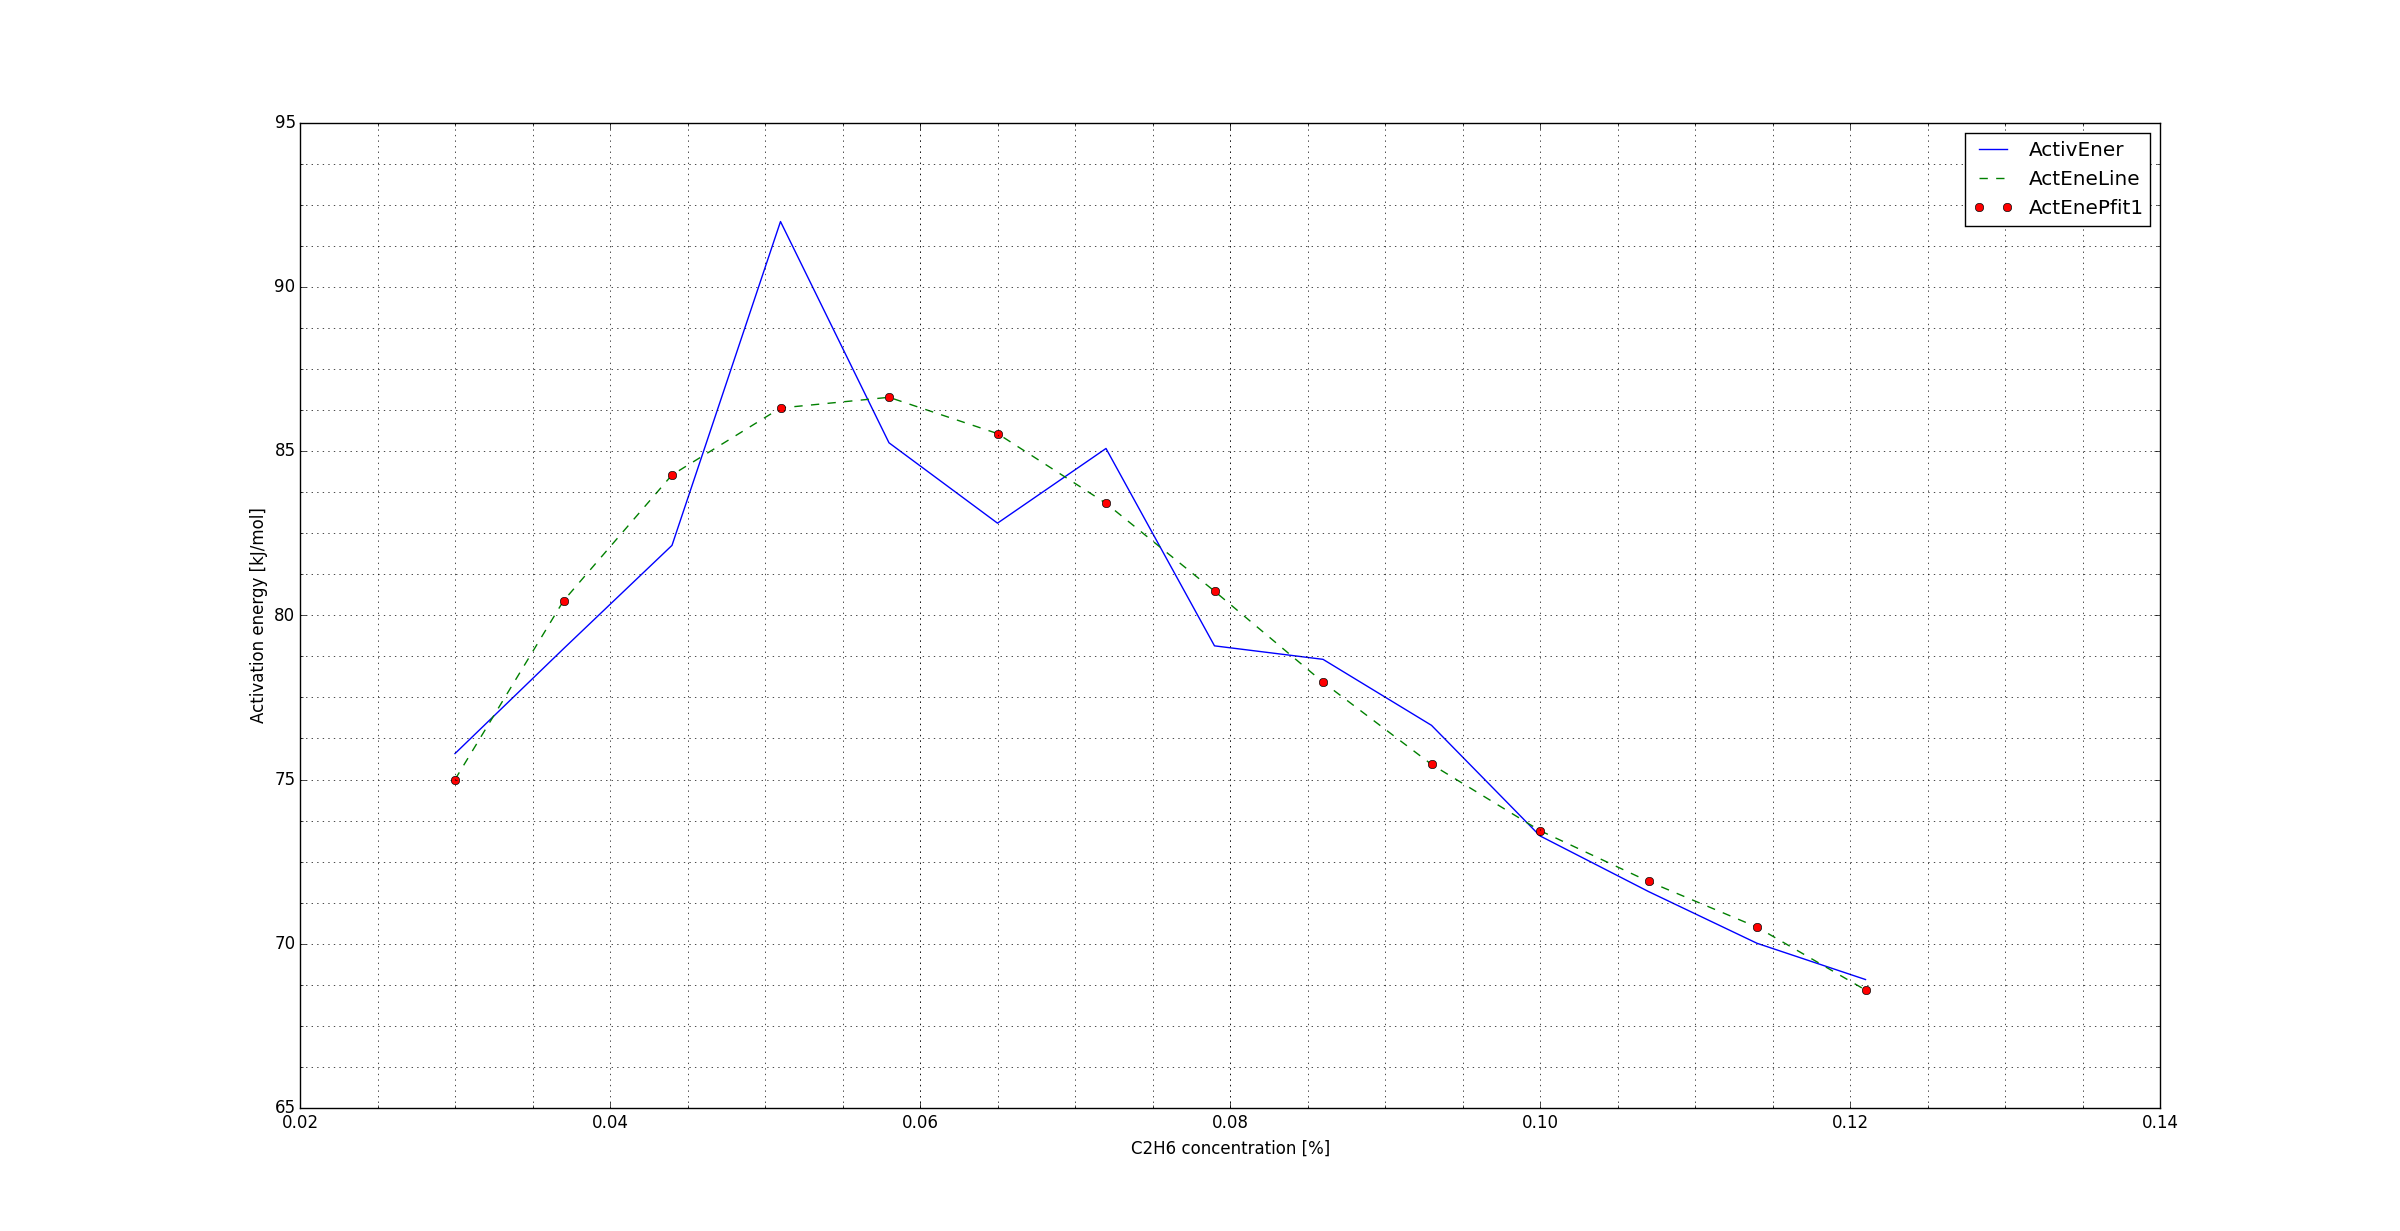
\includegraphics[width=1\textwidth]{figure_2.png}
\caption{Activation energy  at 300 K and 2 atmosphere pressure}
\end{figure}

\hspace{5,5mm} c)Activation energy  at 400 K and 1 atmosphere pressure
\begin{figure}[ht]
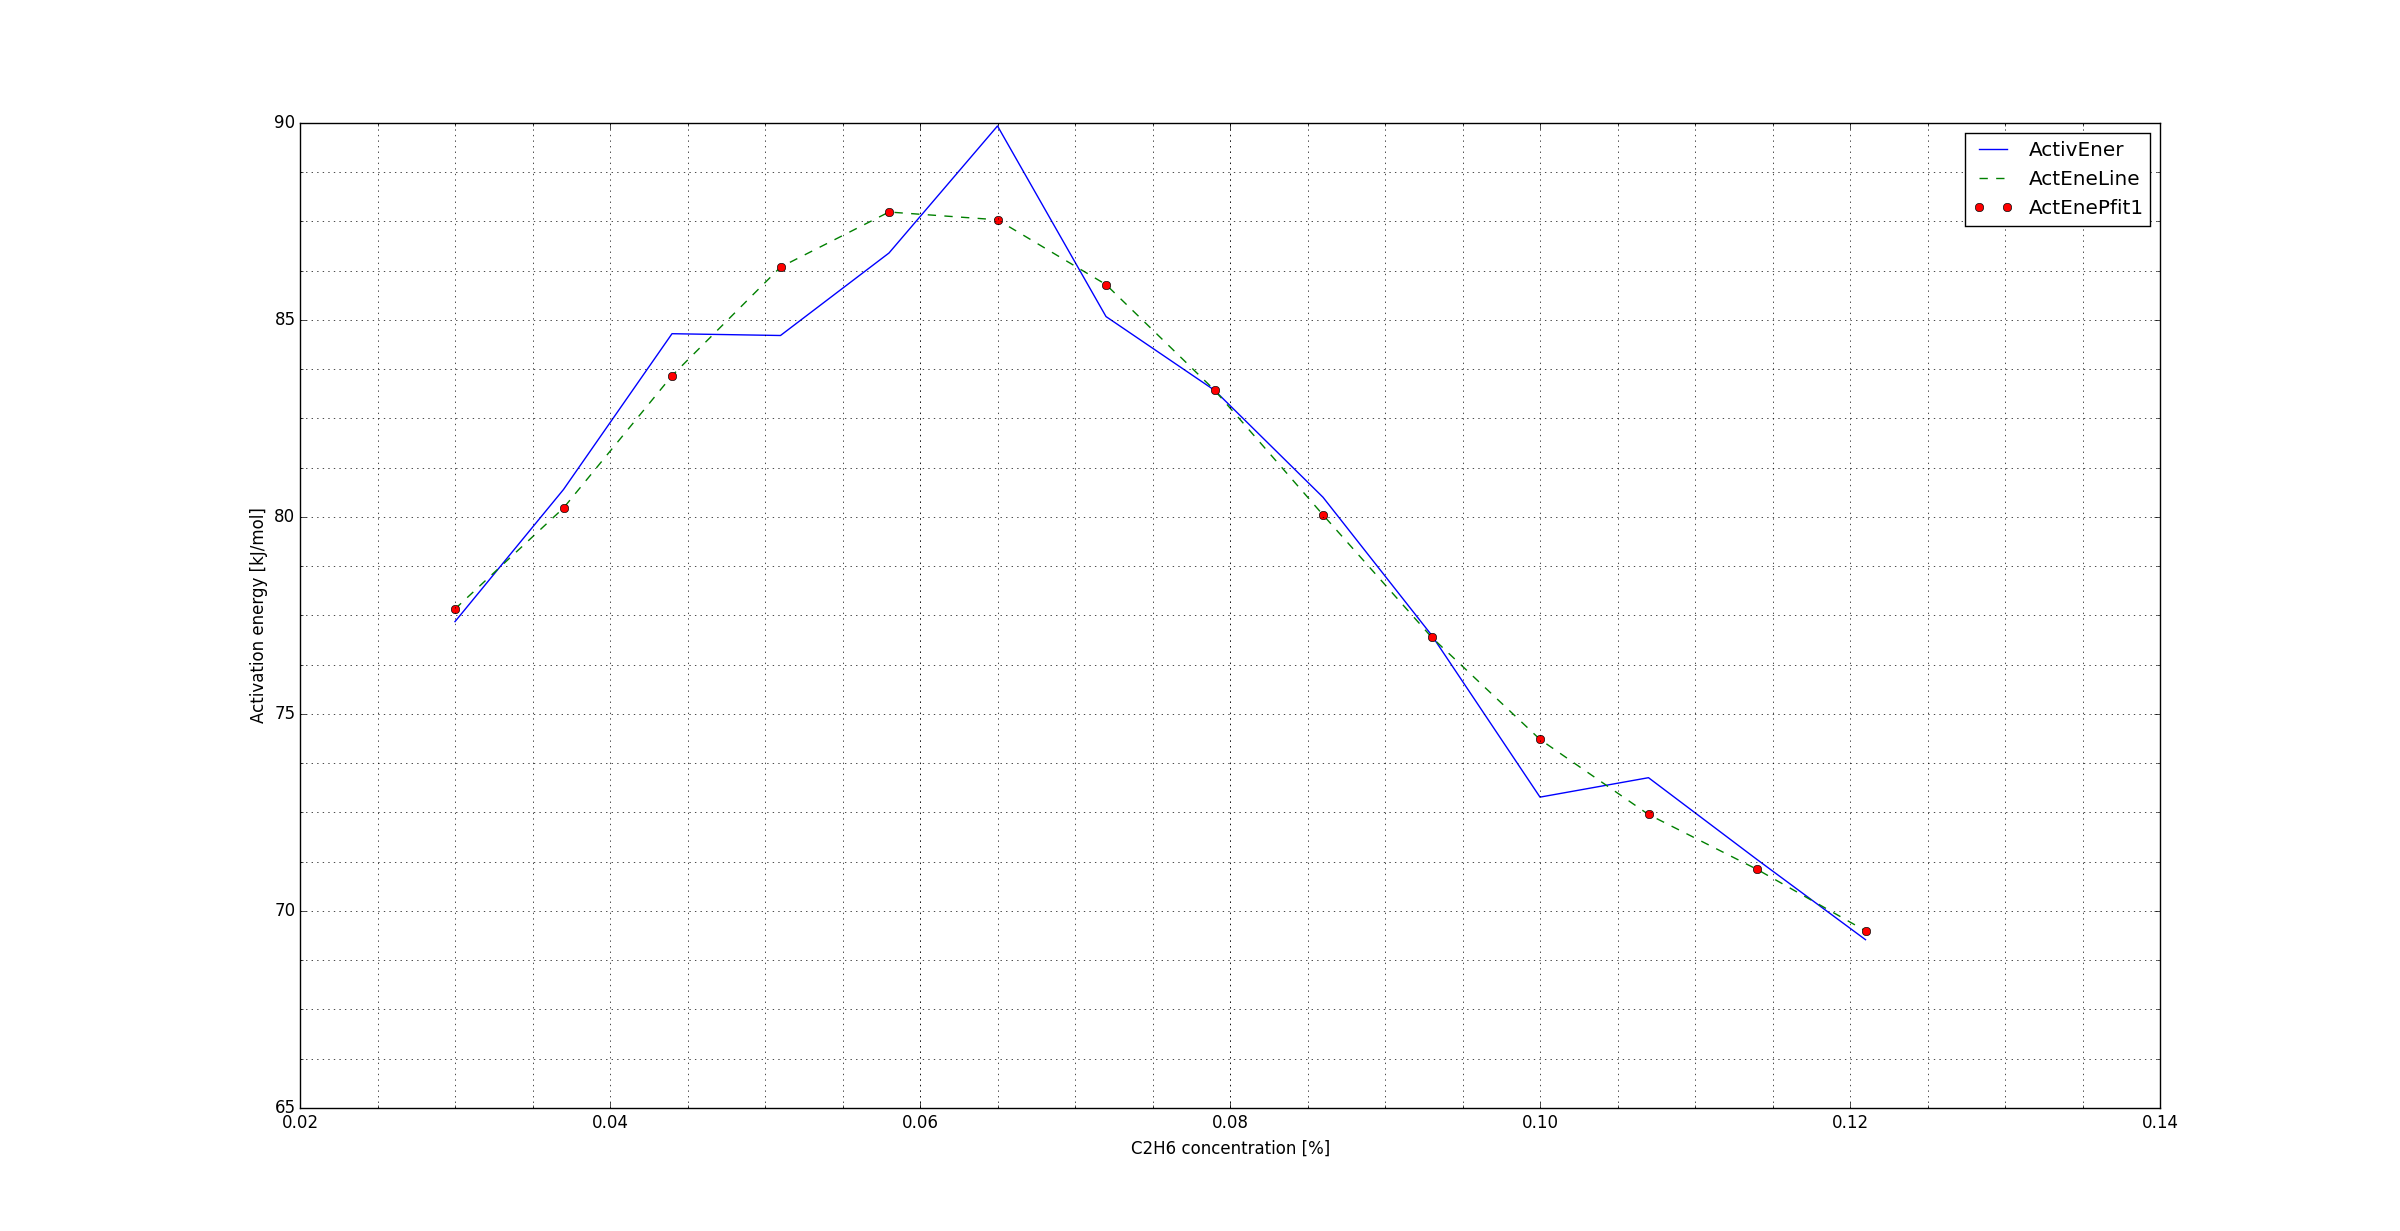
\includegraphics[width=1\textwidth]{figure_3.png}
\caption{Activation energy  at 400 K and 1 atmosphere pressure}
\end{figure}

\hspace{5,5mm} d)Activation energy  at 400 K and 2 atmosphere pressure

\begin{figure}[ht]
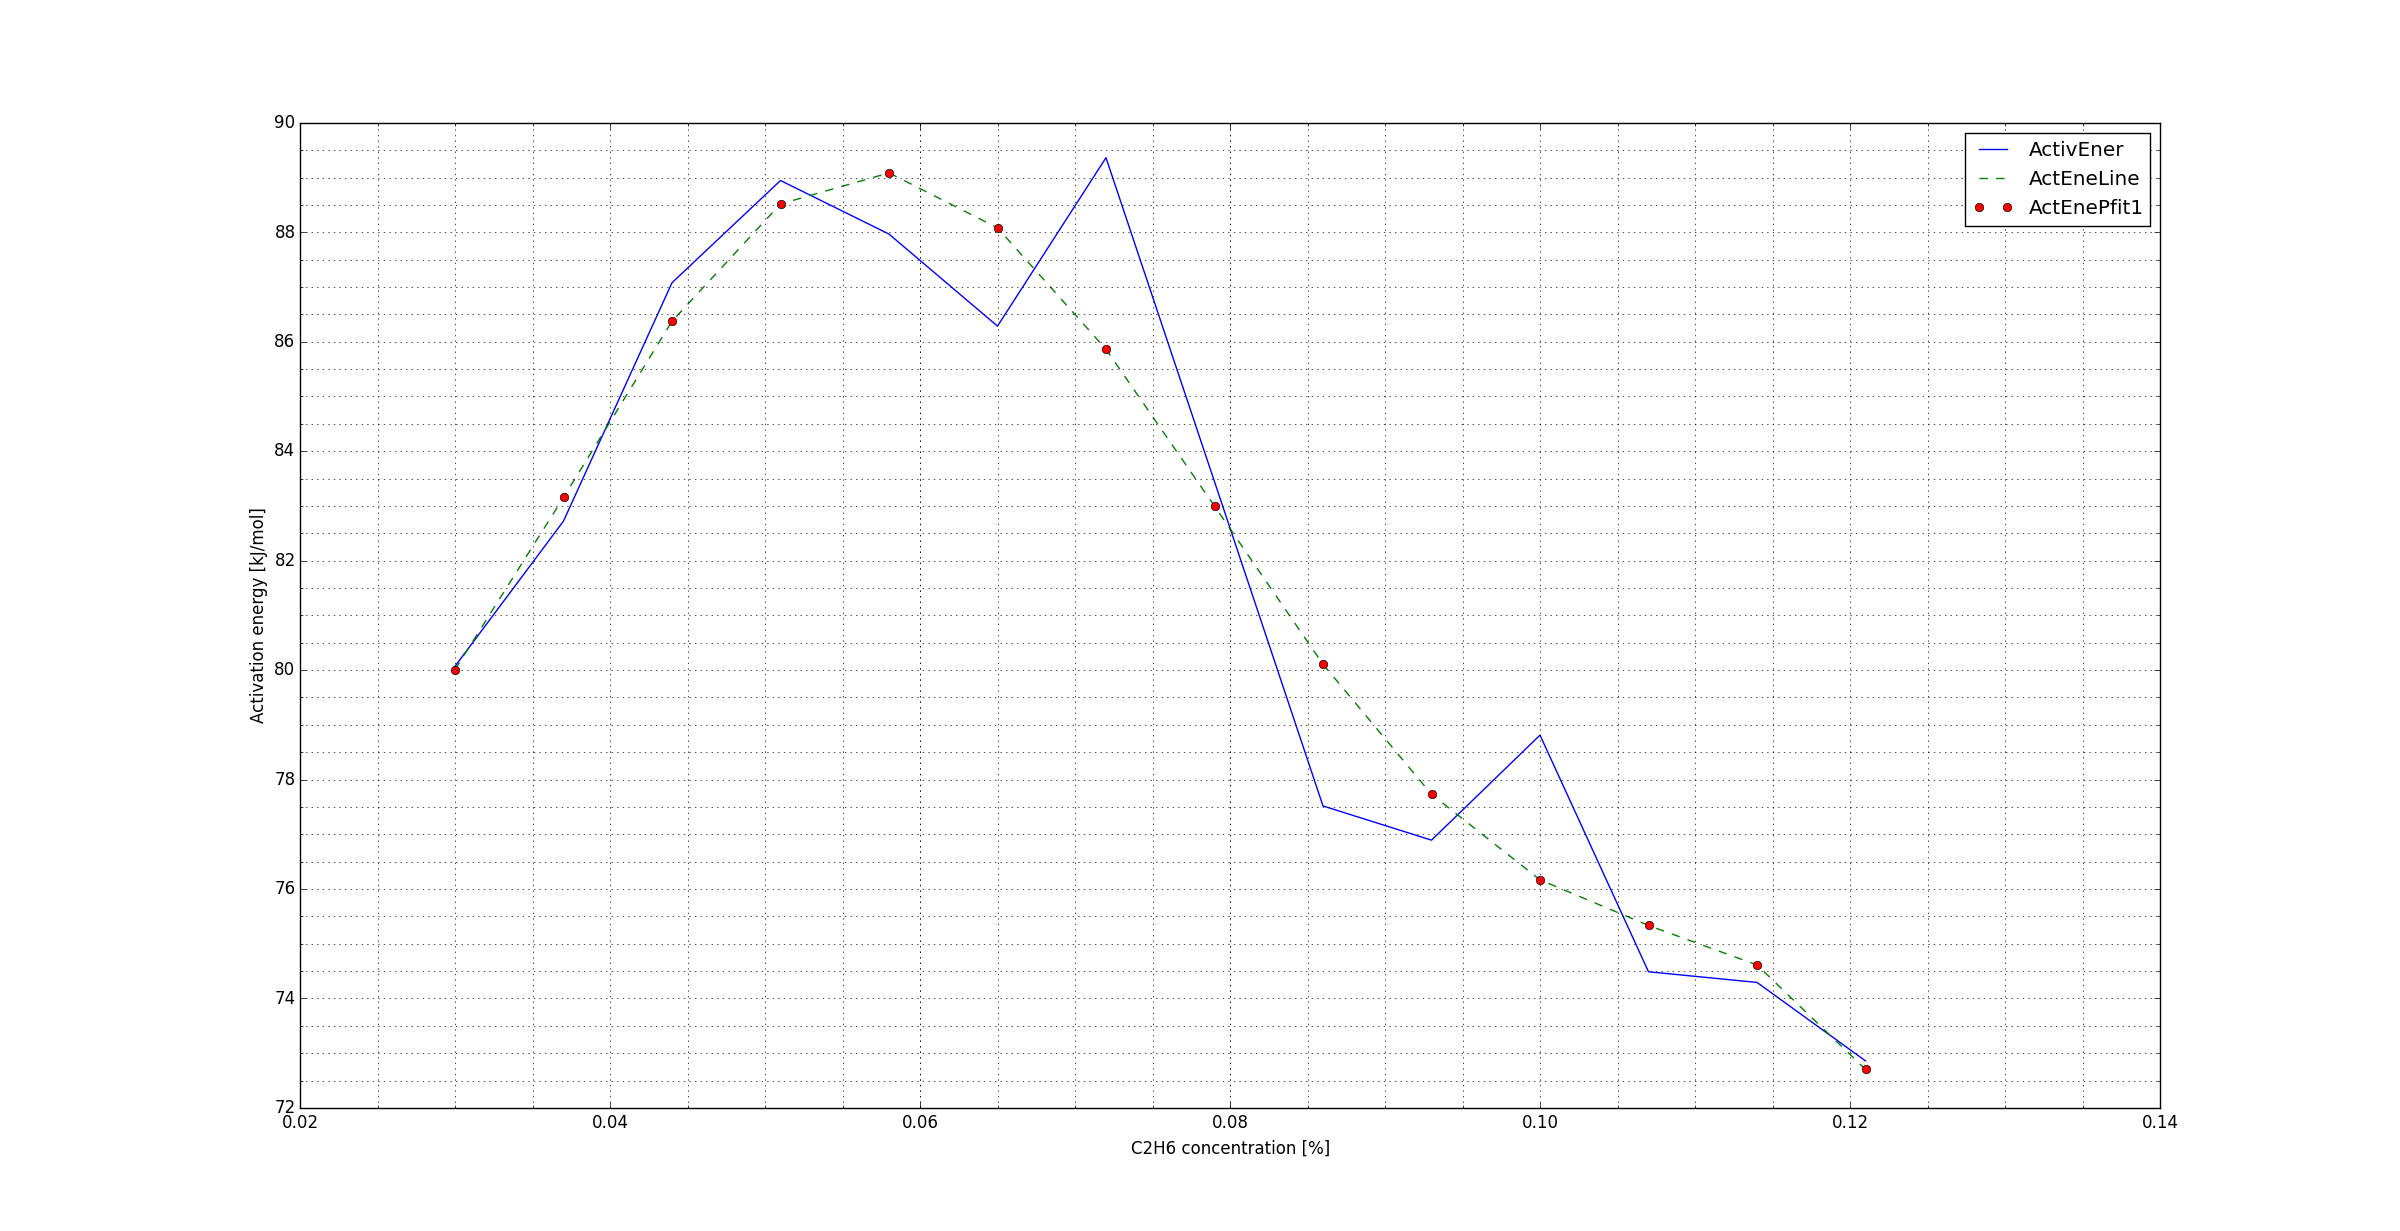
\includegraphics[width=1\textwidth]{figure_4.png}
\caption{Activation energy  at 400 K and 2 atmosphere pressure}
\end{figure}




\section{Summary}
The results for higher temperatures and/or pressures should be significally lesser than corresponded at lower pressure/temperature .However , the outcome seems to be at the safe side of the margin of aberration (values lower than experimental ones), which makes  an output of a program a good initial  approximation for the further research  at explosion safety.






\end{document}